\documentclass[12pt,letterpaper]{article}
\usepackage{color}
\usepackage{graphicx}
\usepackage{geometry}
\usepackage{setspace}
\usepackage{anyfontsize}
\usepackage{parskip}
\usepackage{indentfirst}
\usepackage{amsmath}
\usepackage{natbib}
\usepackage{float}
\usepackage{subcaption}

\geometry{letterpaper, portrait, margin=1in}
\doublespace
\title{On Tessellation and Euclidean Patterns of Polygons}
\author{Tynan Purdy}
\date{\vspace{-5ex}}
\graphicspath{{../images/}}

\begin{document}
\large
\parindent=0.5in
{\fontsize{12}{14.4}
	{\singlespace
	\pagenumbering{gobble}
	\maketitle
	\begin{center}
	\vspace{4mm}
	002129-0004 \\
	\vspace{4mm}
	IB Math HL IA \\
	\vspace{4mm}
	May 2019 \\
	\vspace{4mm}
	Words: 1033\\
	\end{center}
	}
}	

\newpage
\pagenumbering{arabic}
\begin{abstract}
Tessellation is the bridge between art and mathematics. It is the uniform patterning of a shape over a plane with no gaps between individual instances of the shape. Tessellations have existed in art and in architecture for thousands of years, dating back to early Islam \citep{arabic}. I am personally interested in tessellated patterns because they are relevant and applicable to graphic design and mechanical engineering. I use tessellations in SolidWorks Computer-Aided Design (CAD) software for mechanical design and Adobe Illustrator\textsuperscript{\textregistered} for graphic and art projects. Both programs have functions for generating tessellations, and the methods behind those functions will be explored.
\end{abstract}

\newpage
\tableofcontents

\newpage
\section{Introduction}
Tessellation is everywhere. In a carpentered, geometric world, patterns of polygons make up many structures and visual elements around us, from ceiling tiles to brick sidewalks. Their advantages are well suited for filling an area in a way that is both efficiently achievable from a manufacturing and installation standpoint, and being visually appealing. Regularly patterning one shape means only one part has to be made. Minimizing the number of configurations of a part drastically improves the ability to produce that part at scale. The fewer processes required to produce a part can also lower the cost of production. In the industrialized world, qualities like these have made tessellation an extremely commonly used tactic in design of all kinds. Since tessellation is such a prominent occurrence, it should be understood what tessellation is, where it came from and how it is performed mathematically.

\subsection{Historic Origins}
Some of the oldest known implementations of tessellation patterns are in Islamic art. Carpets and ornamental decorations in Mosques are littered with unique geometric patterns. 

\begin{figure}[H]
    \begin{center}
        \caption{Artistic tessellations in the style of traditional Islamic art.}
        \label{fig:islam}
        \begin{subfigure}[b]{.3\linewidth}
            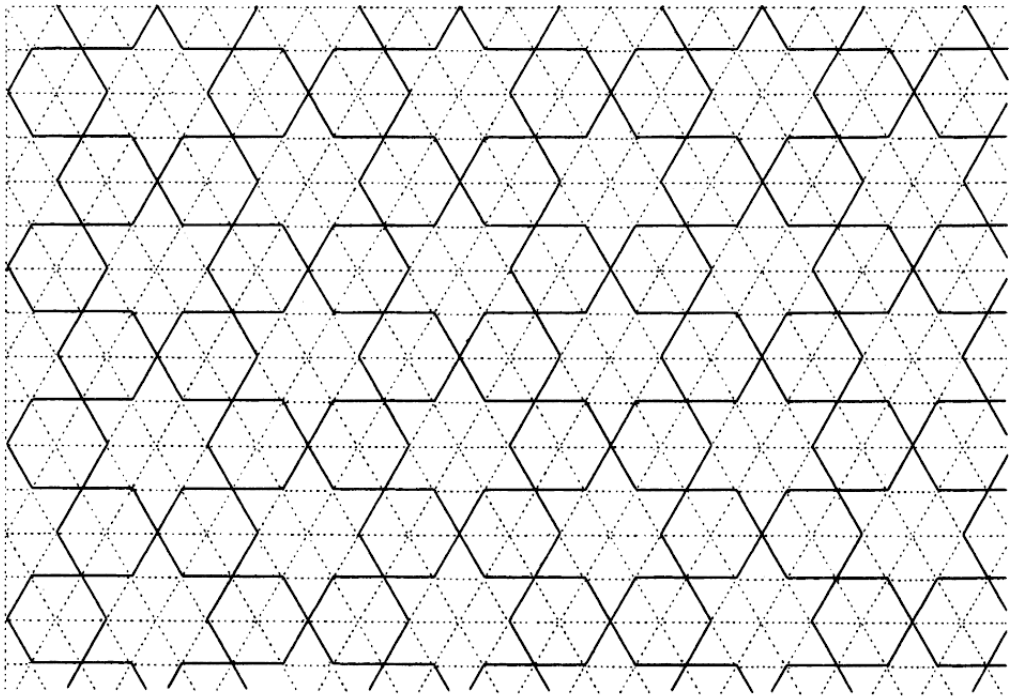
\includegraphics[width=\linewidth]{islam1}
        \end{subfigure}
        \begin{subfigure}[b]{.3\linewidth}
            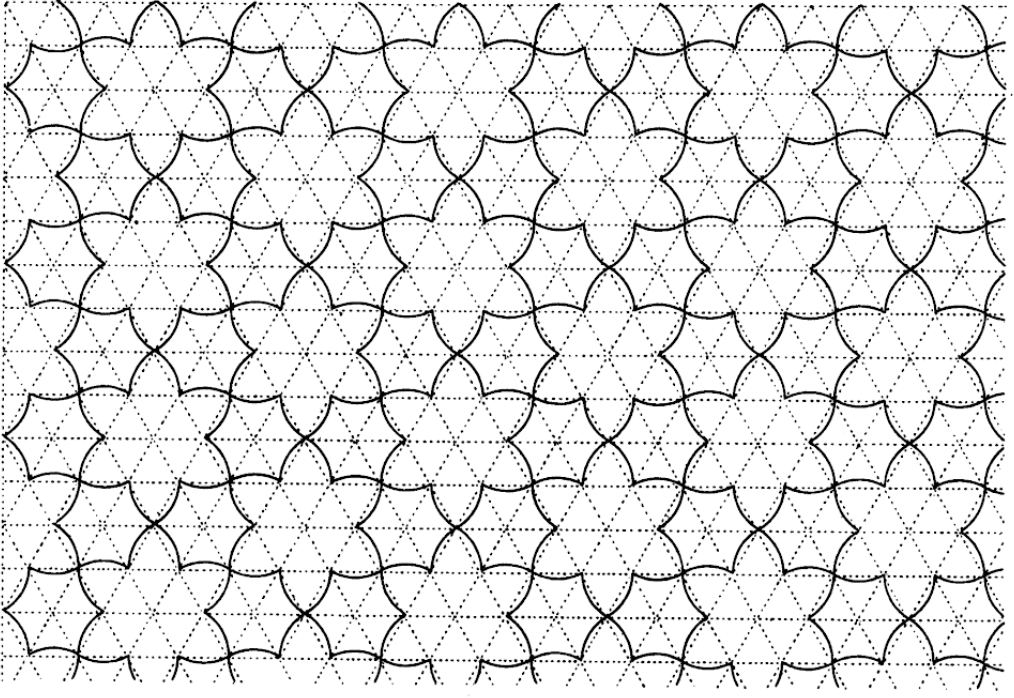
\includegraphics[width=\linewidth]{islam2}
        \end{subfigure}
        \begin{subfigure}[b]{.3\linewidth}
            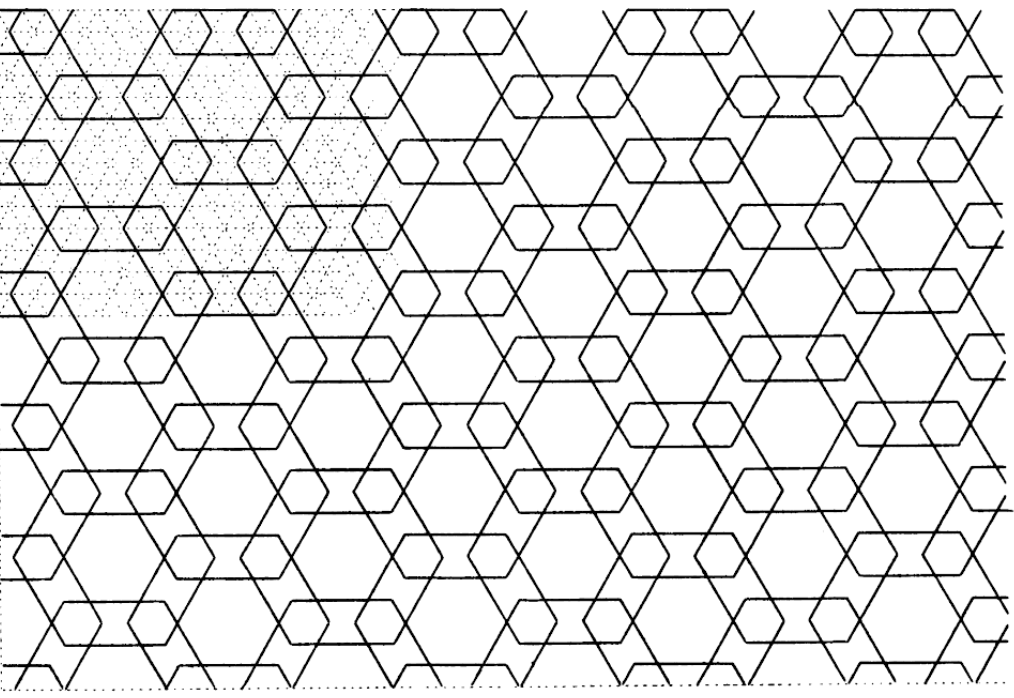
\includegraphics[width=\linewidth]{islam3}
        \end{subfigure}
    \end{center}
\end{figure}

There are multiple styles of Islamic polygon patterning, one of which is Girih tiles. Girih tiles were used in the 15th century to decorate Persian Islamic buildings \citep{girih}. There are five different polygons used in a Girih tile. As with the hexagonal tessellations, the patterned polygon is often hidden, while the artistic lines within each shape are shown to display the pattern.

\begin{figure}[H]
    \begin{center}
        \label{fig:girih}
        \caption{Girih base tiles and tessellation}
        \begin{subfigure}[b]{.5\linewidth}
            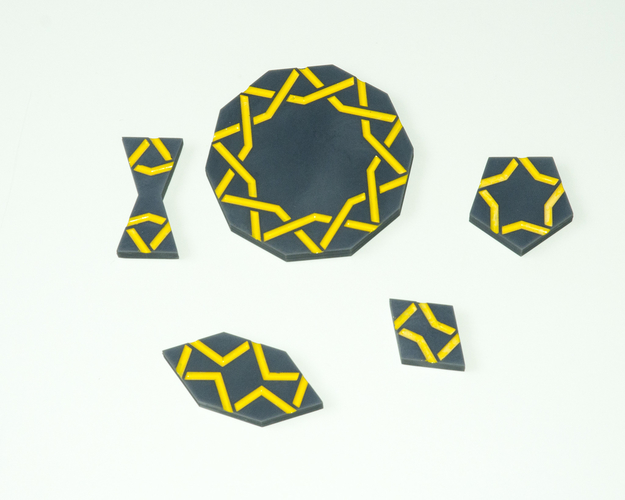
\includegraphics[width=\linewidth]{3dgirih}
            \caption{3D printed Girih tiles, designed by pinshape user mgarrity.}
            \label{fig:3dgirih}
        \end{subfigure}
        \begin{subfigure}[b]{.4\linewidth}
            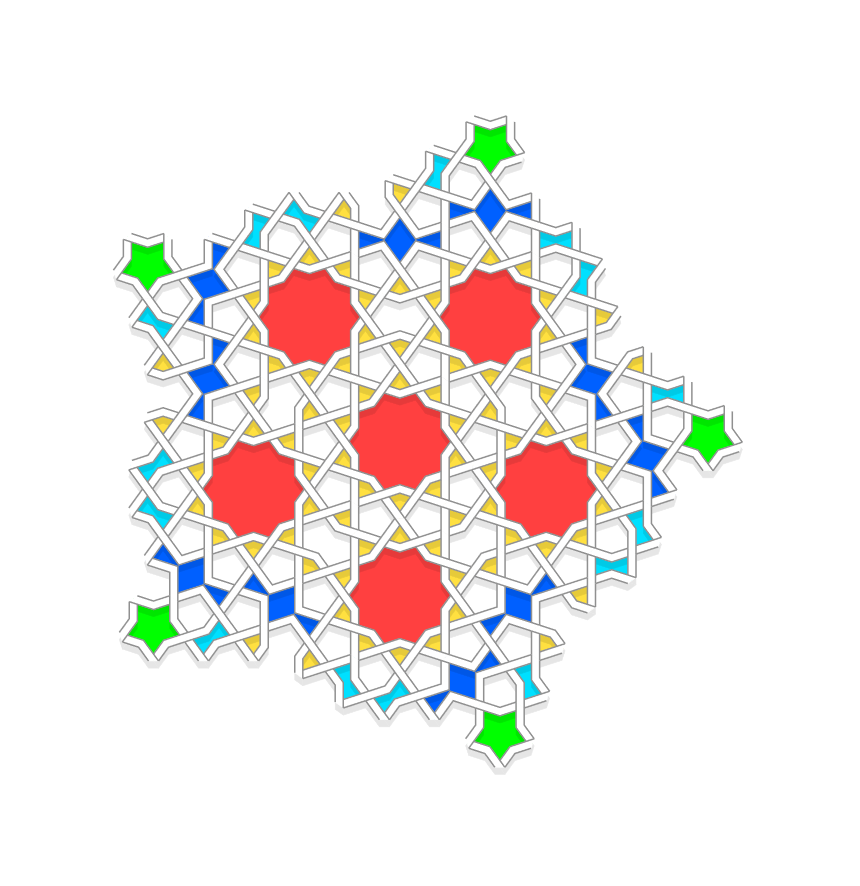
\includegraphics[width=\linewidth]{girih-art}
            \caption{Girih tiling example, created with girihdesigner.com}
            \label{fig:girihex}
        \end{subfigure}
    \end{center}
\end{figure}

Figure \ref{fig:3dgirih} shows the five base Girih polygons. The yellow lines are an artistic pattern added on top of the polygons. An example of an implemented Girih tiling is shown in figure \ref{fig:girihex}.

\section{Tessellation}
Tessellations are described using the notation of the Schl\"afli symbol (\ref{eq:schlafli}), where $p$ is the number of edges and $q$ is the number of edges intersecting at a vertex.

\begin{equation}
    \label{eq:schlafli}
    \{p,q\}
\end{equation}

A tessellation must follow certain rules. There may be no gaps between different tiles, or polygons, and there may be no vertices on an edge. There are 3 periodic Euclidean 2D tessellations using a single convex polygon with no gaps that can be patterned infinitely on the 2D plane: rectangular grids, honeycombs, and triangular grids. These are by far the most commonly found tessellations.

\begin{figure}[H]
    \begin{center}
        \caption{Tessellation of rectangle $\{4,4\}$}
        \label{fig:square}
        \begin{subfigure}[b]{.3\linewidth}
            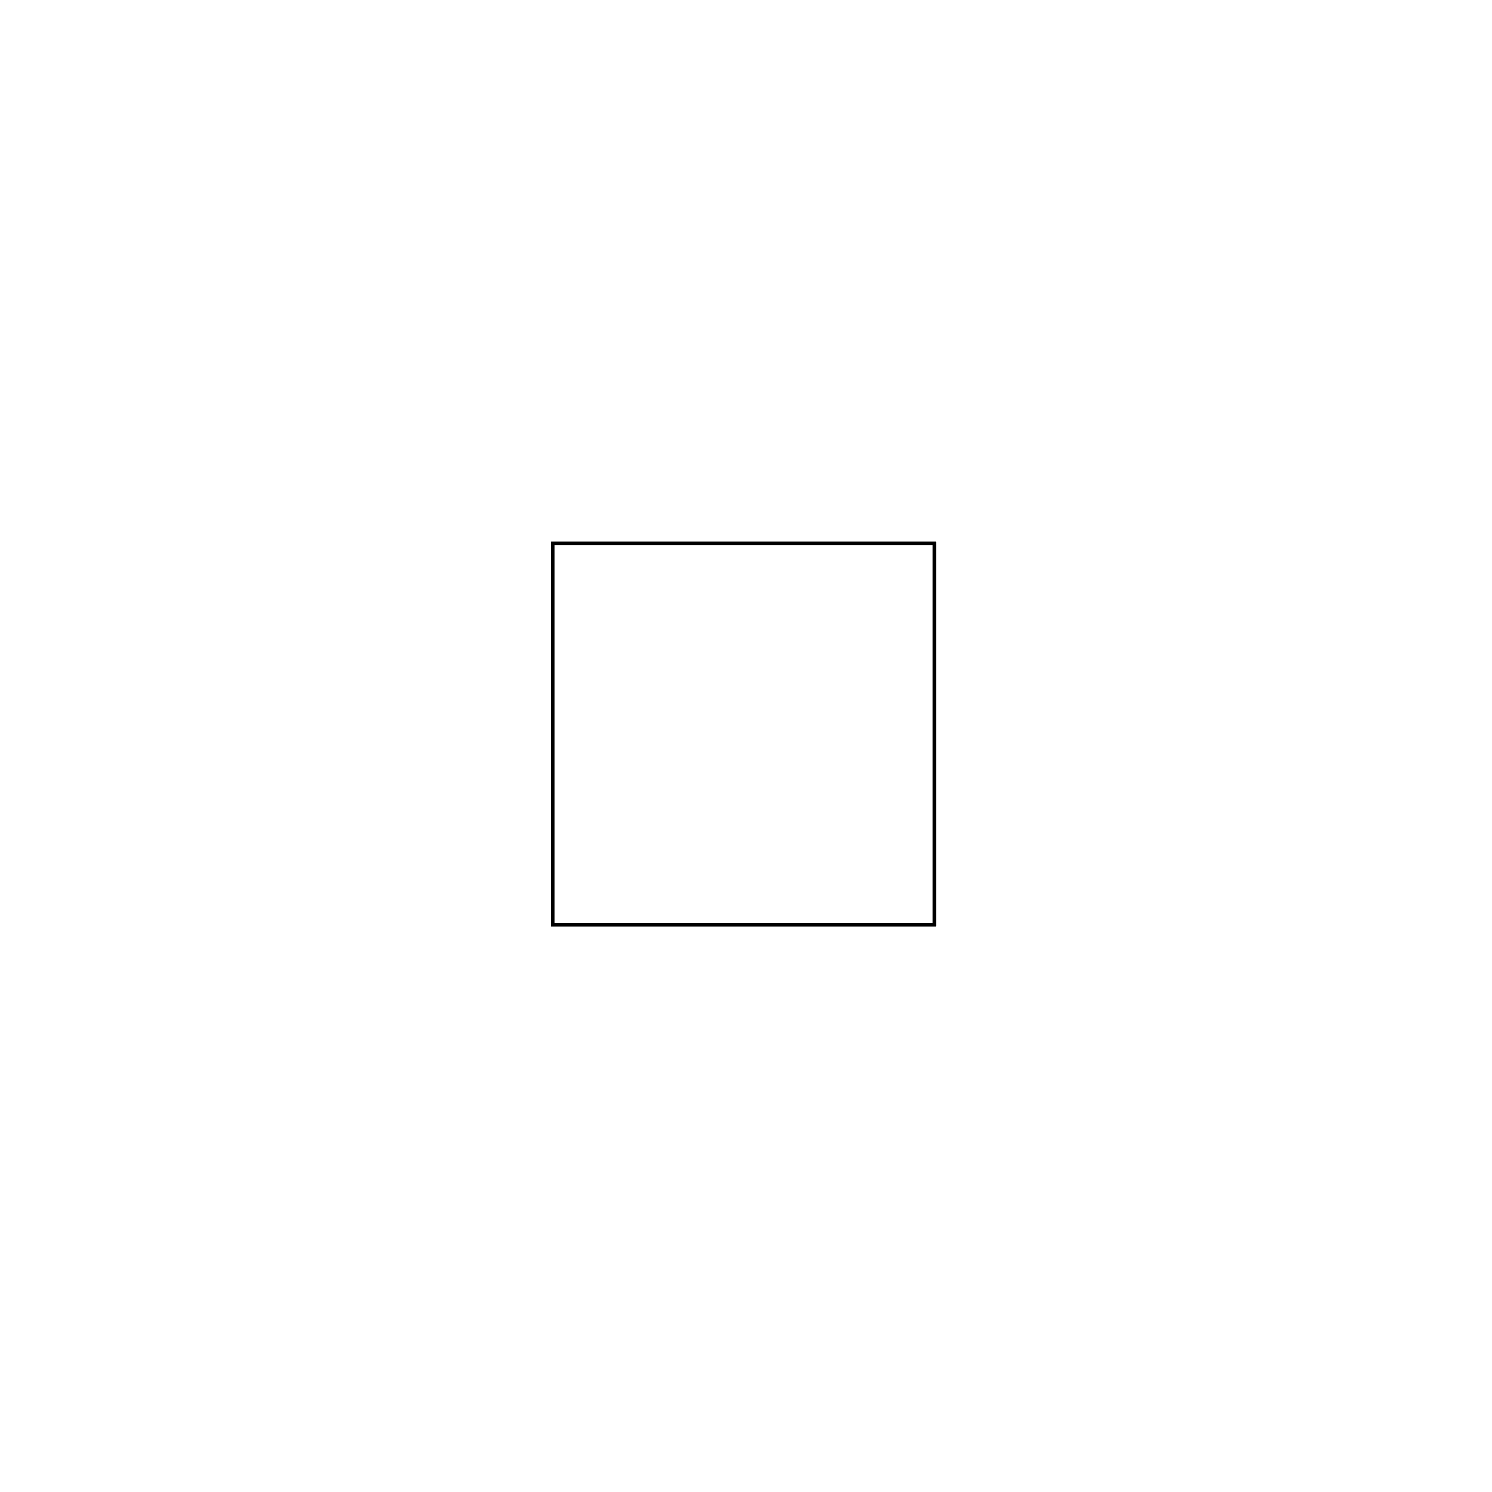
\includegraphics[width=\linewidth]{base-square}
            \caption{Base 4-sided shape}
        \end{subfigure}
        \begin{subfigure}[b]{.3\linewidth}
            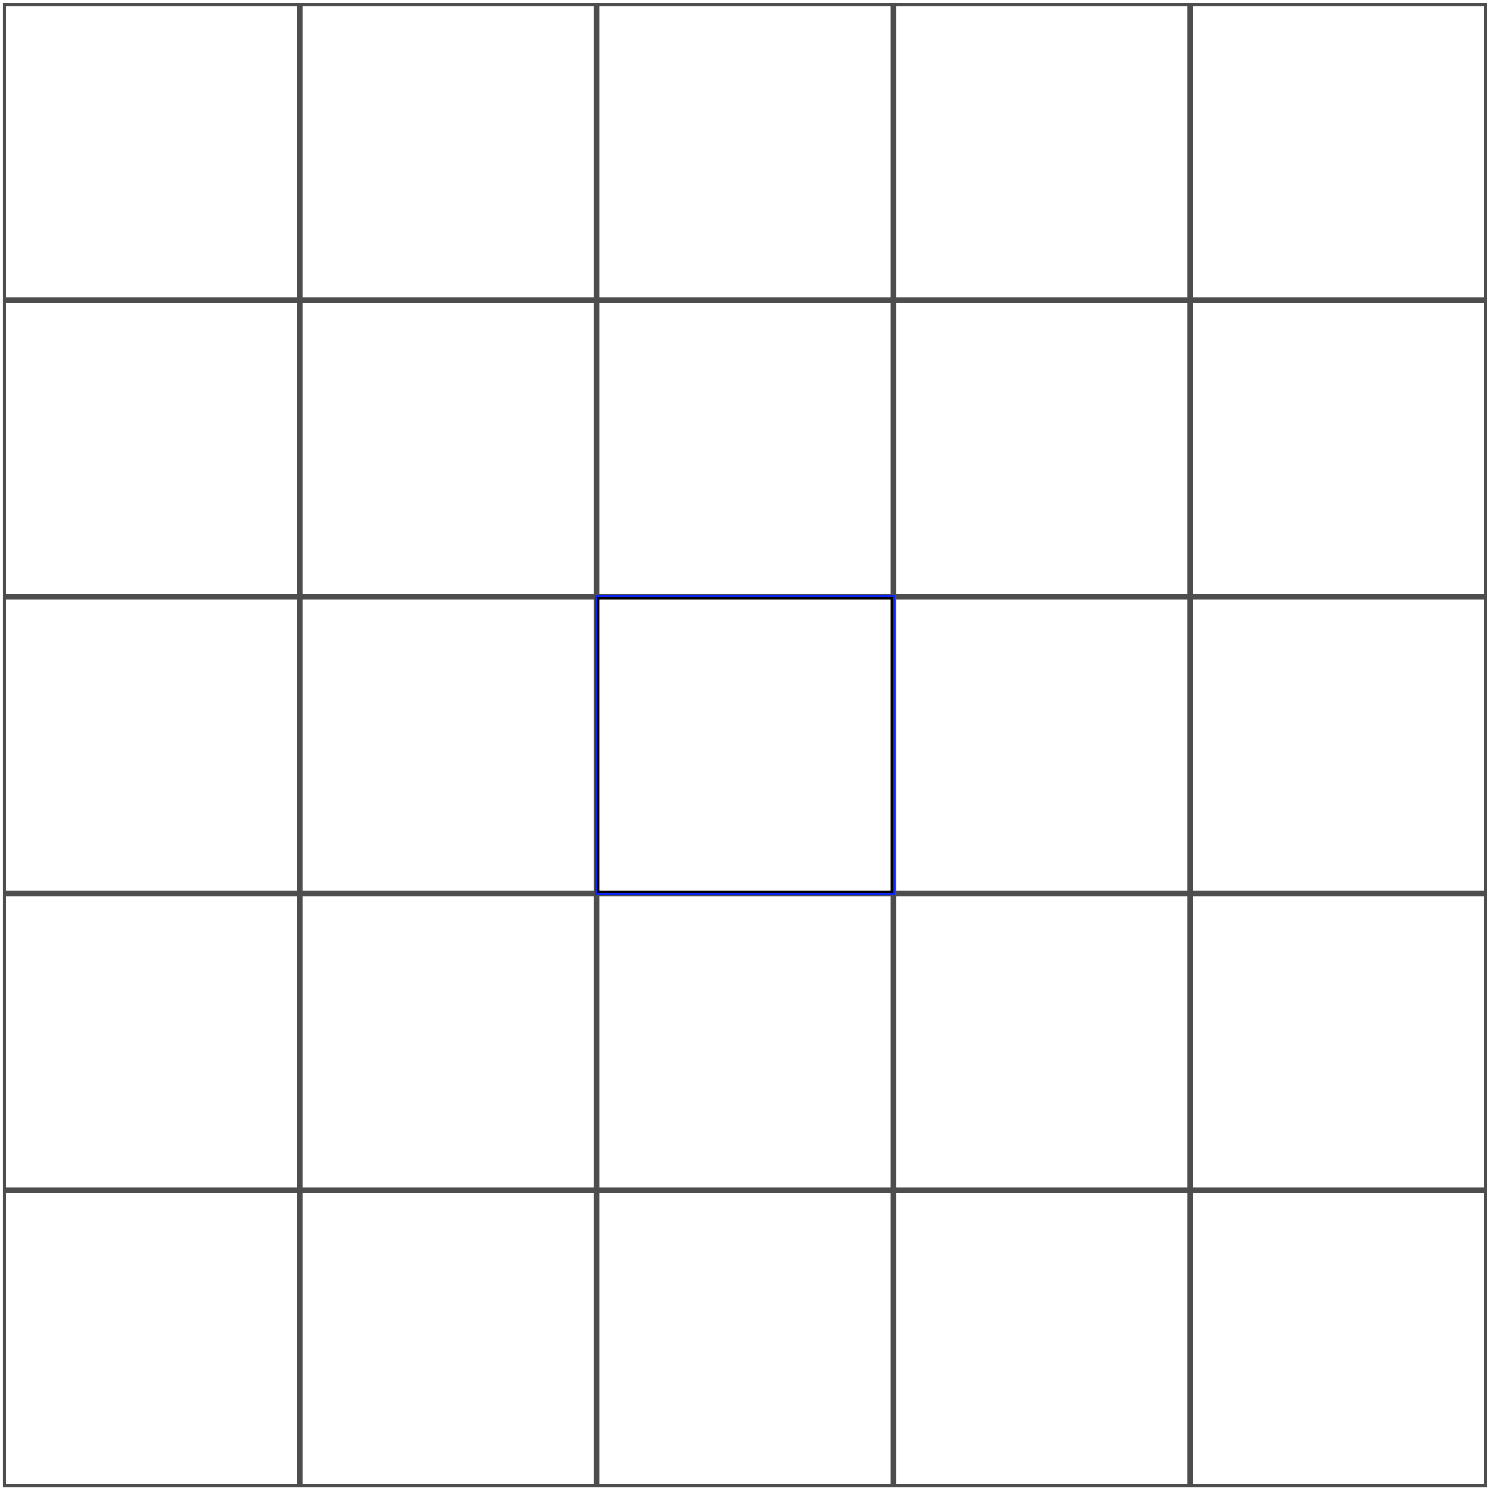
\includegraphics[width=\linewidth]{tes-square}
            \caption{5x5 tessellation}
        \end{subfigure}
    \end{center}
\end{figure}

\begin{figure}[H]
    \begin{center}
        \caption{Tessellation of a hexagon, also known as a honeycomb $\{6,3\}$}
        \label{fig:hex}
        \begin{subfigure}[b]{.3\linewidth}
            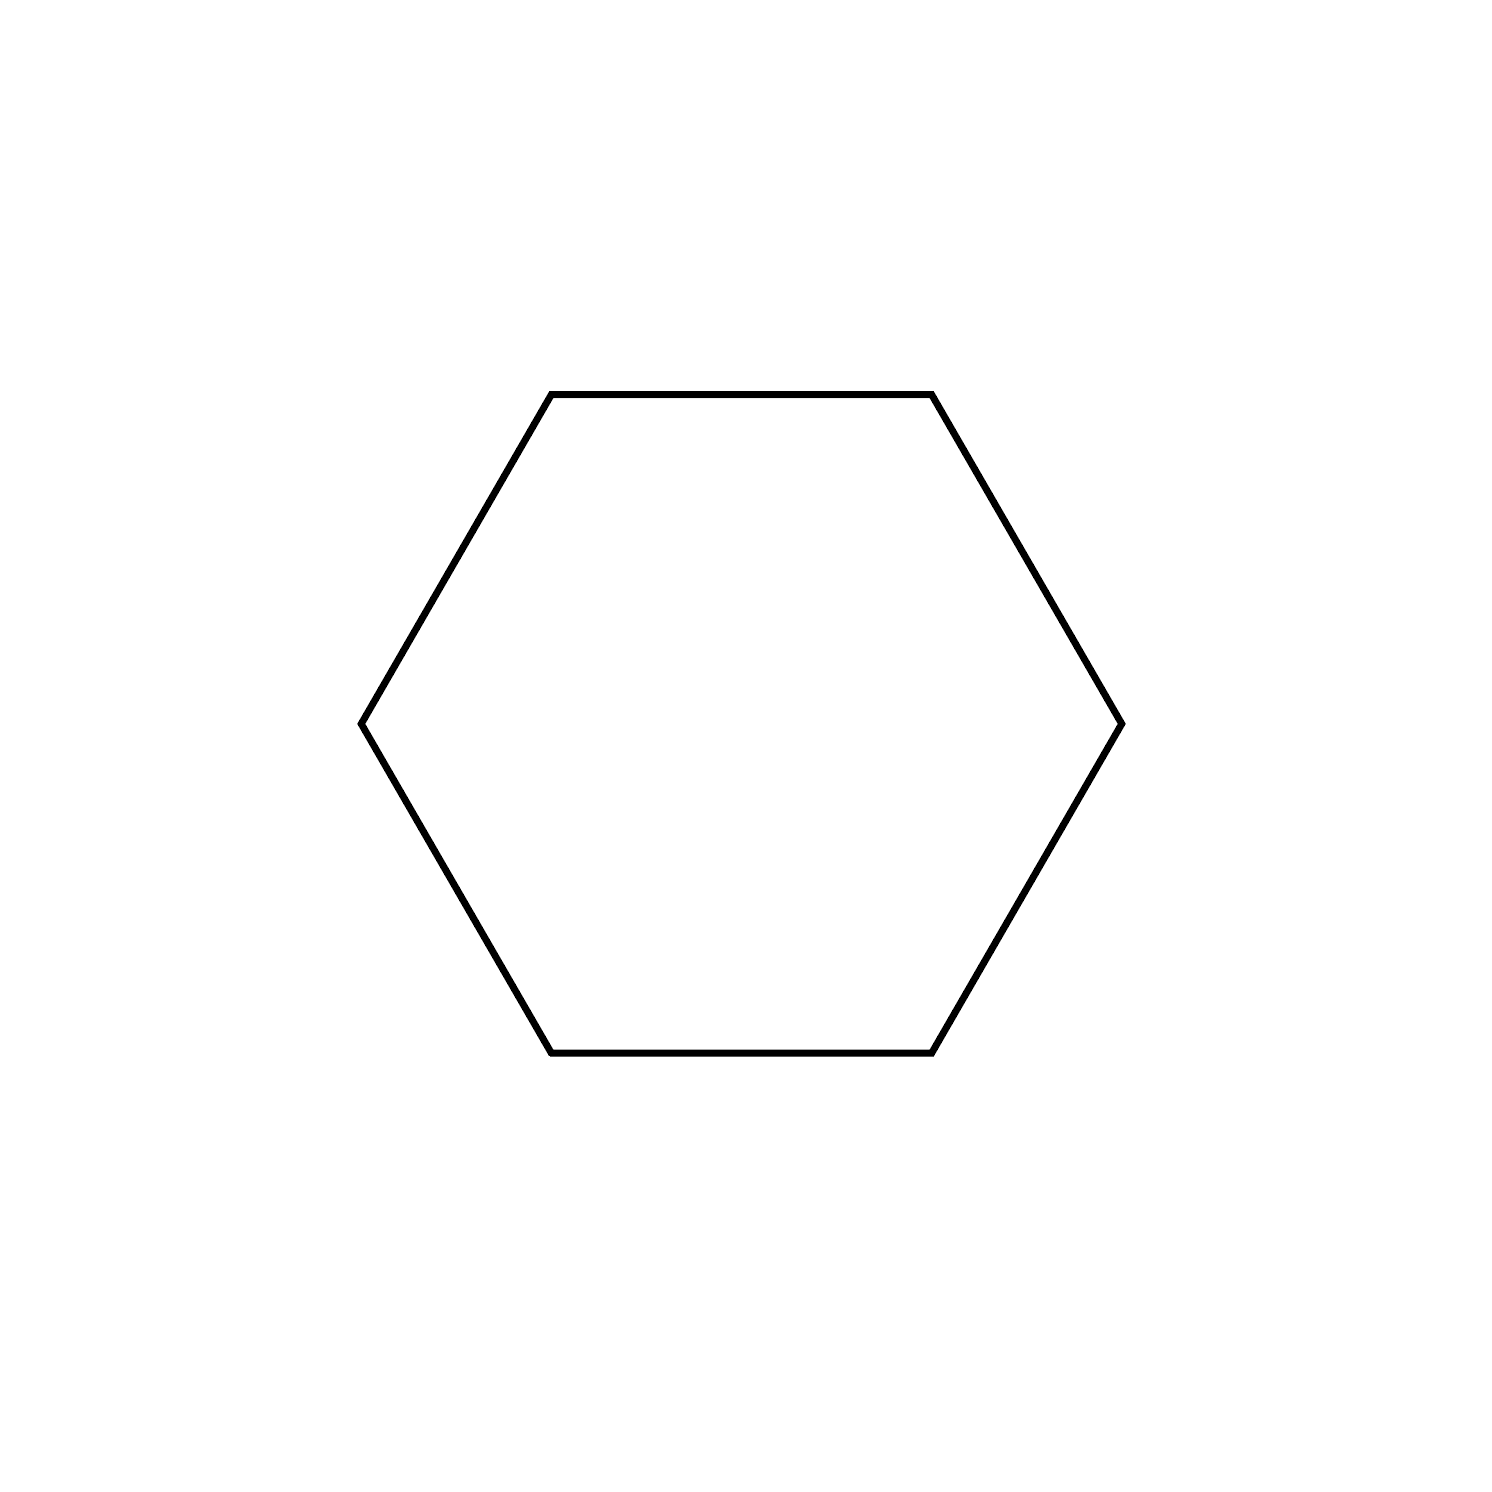
\includegraphics[width=\linewidth]{base-hex}
            \caption{Base 6-sided shape}
        \end{subfigure}
        \begin{subfigure}[b]{.3\linewidth}
            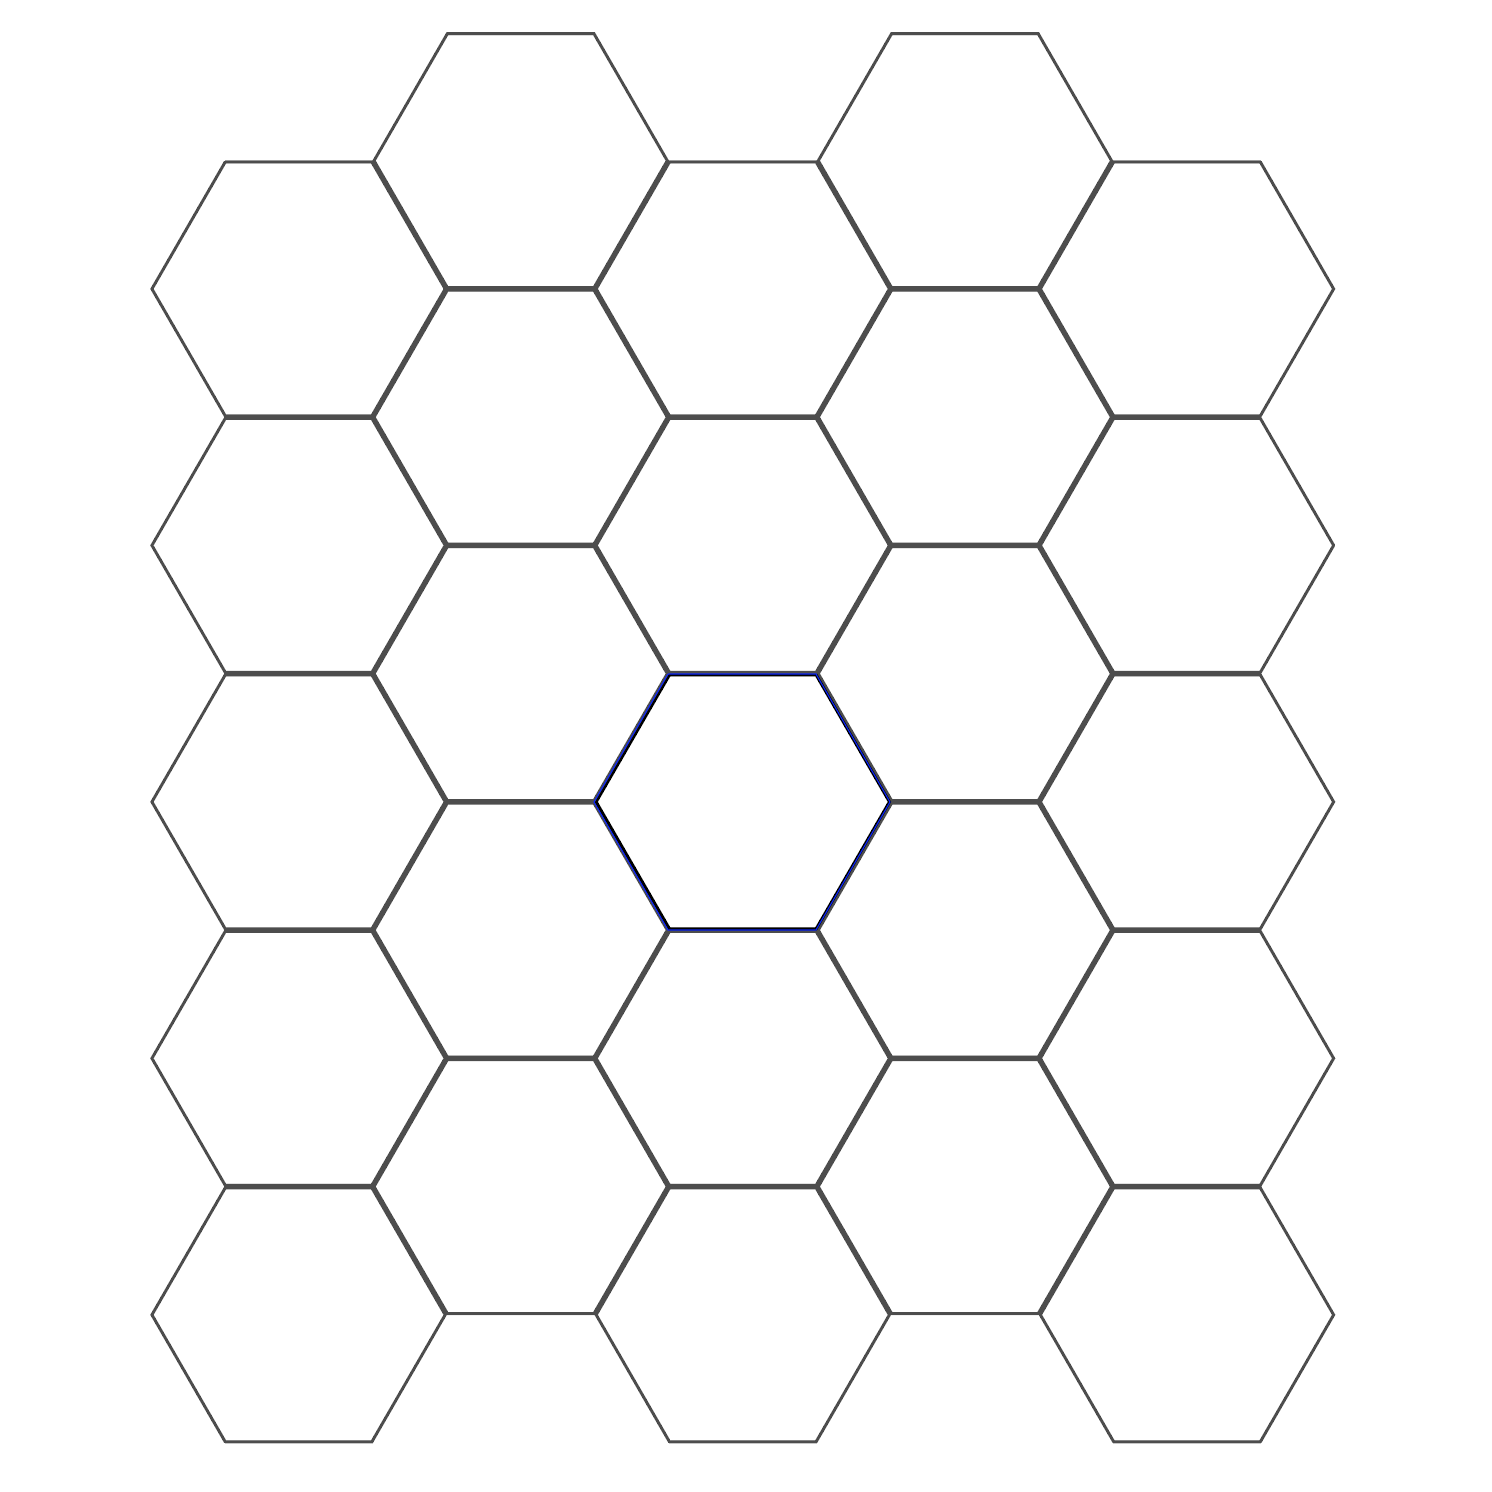
\includegraphics[width=\linewidth]{tes-hex}
            \caption{5x5 tessellation}
        \end{subfigure}
    \end{center}
\end{figure}

\begin{figure}[H]
    \begin{center}
        \caption{Tessellation of a triangle $\{3,6\}$}
        \label{fig:tri}
        \begin{subfigure}[b]{.3\linewidth}
            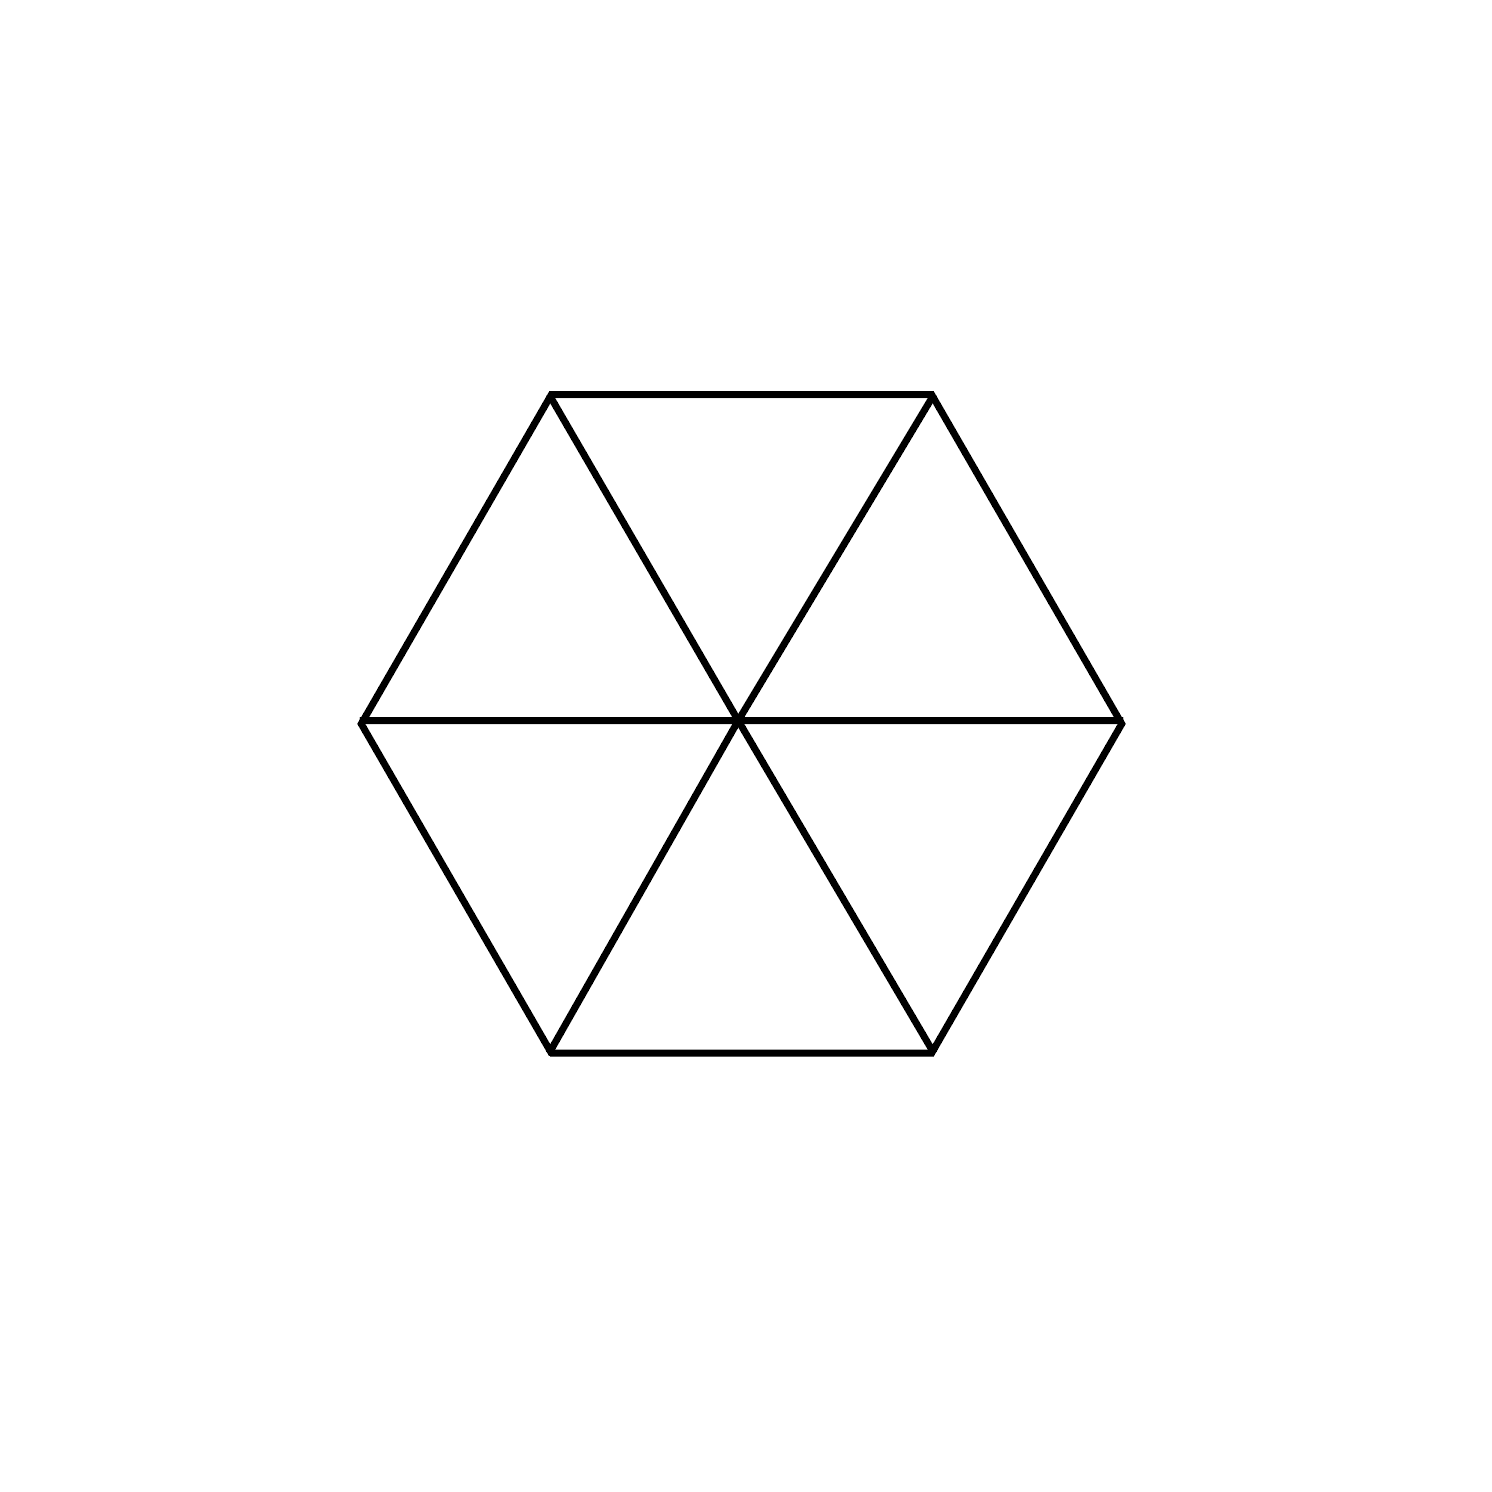
\includegraphics[width=\linewidth]{base-tri}
            \caption{Base 3-sided shape (fits within the base hexagon)}
        \end{subfigure}
        \begin{subfigure}[b]{.3\linewidth}
            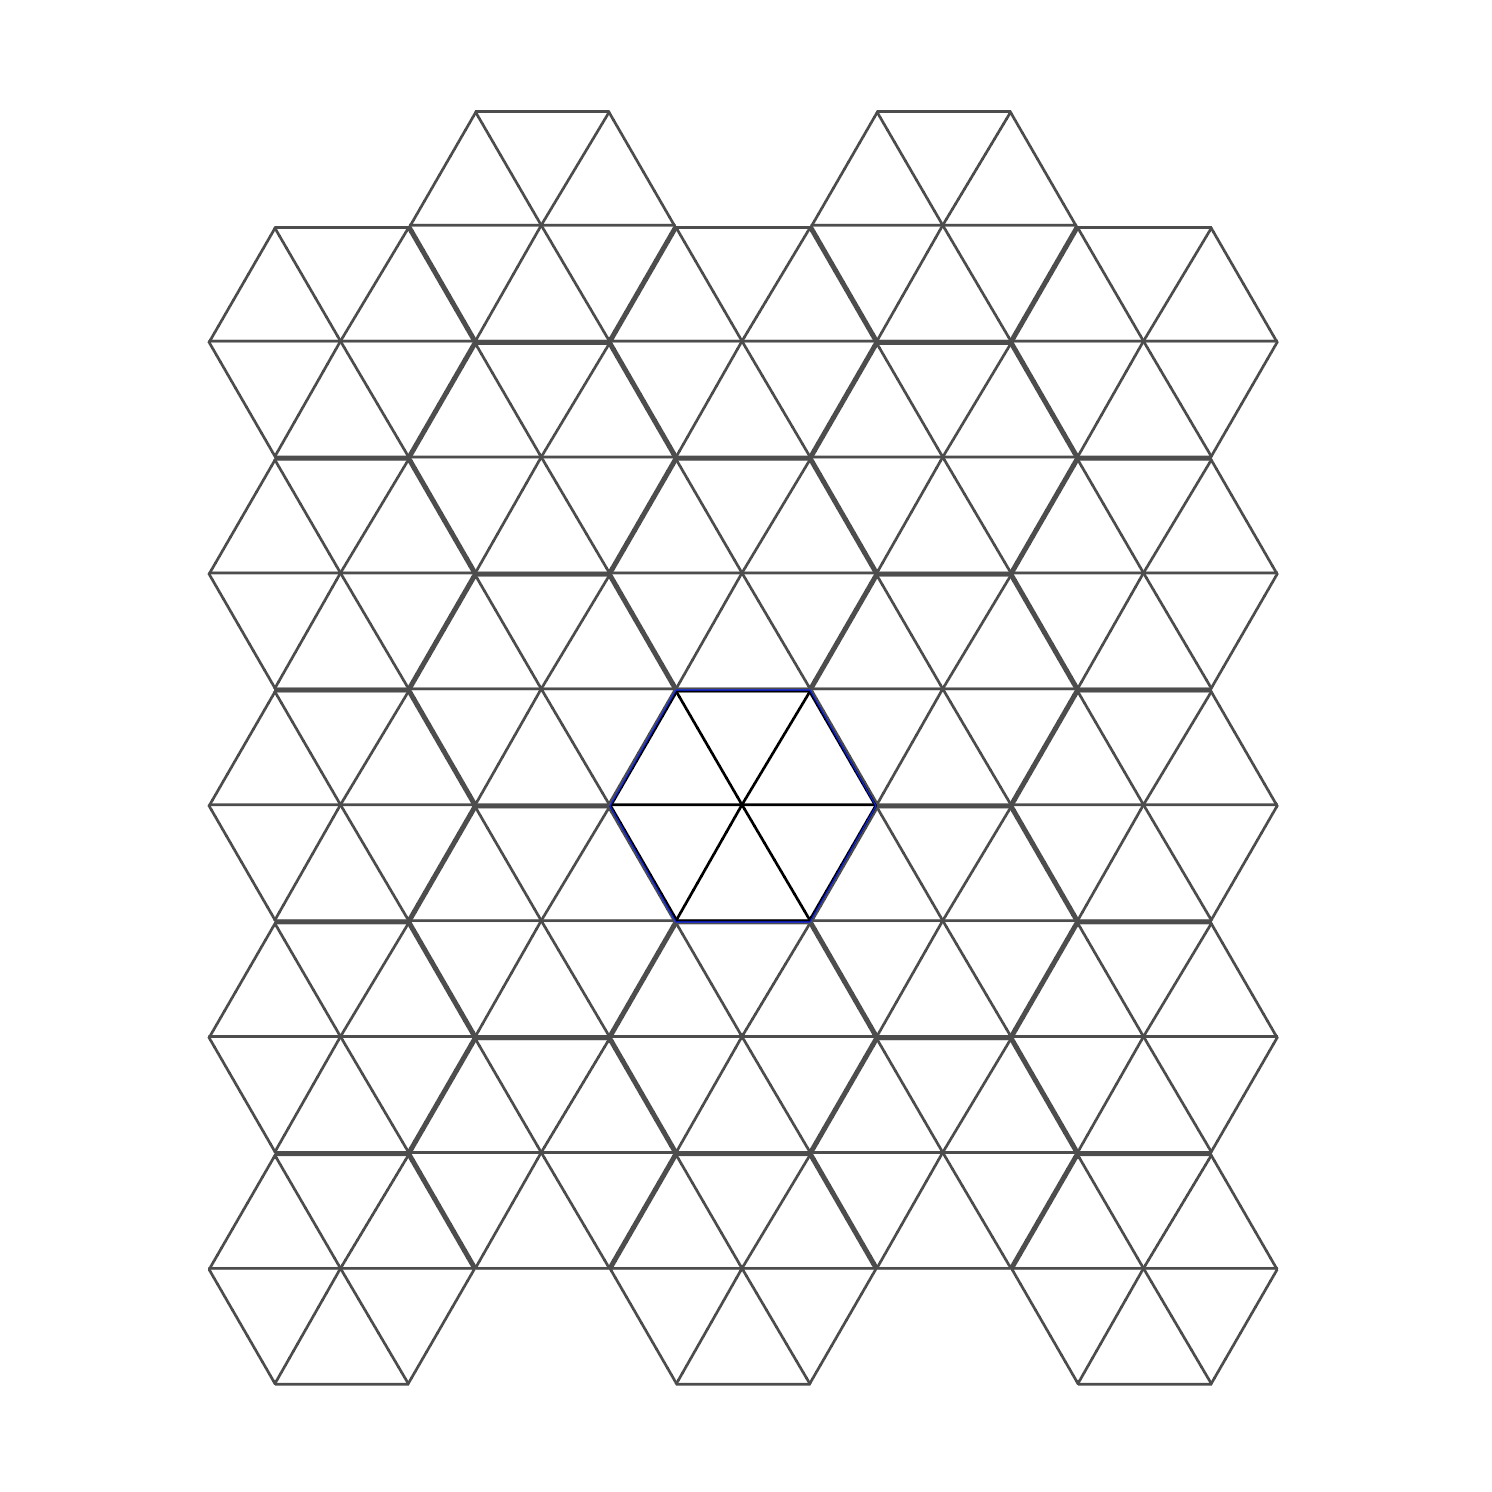
\includegraphics[width=\linewidth]{tes-tri}
            \caption{15x10 tessellation}
        \end{subfigure}
    \end{center}
\end{figure}

It should be noted that many artistic patterns are simply a form of regular tessellation with additional lines and elements within the base shape. For instance, all of the examples of Islamic tessellations in figure \ref{fig:islam} are abstractions of the regular tessellation $\{6,3\}$. Additionally, all of the example tessellations shown in this section (Figures \ref{fig:square}, \ref{fig:hex}, \ref{fig:tri}) were generated using the Adobe Illustrator\textsuperscript{\textregistered} \, ``make pattern'' tool (figure \ref{fig:adobe}).

\begin{figure}[H]
    \begin{center}
        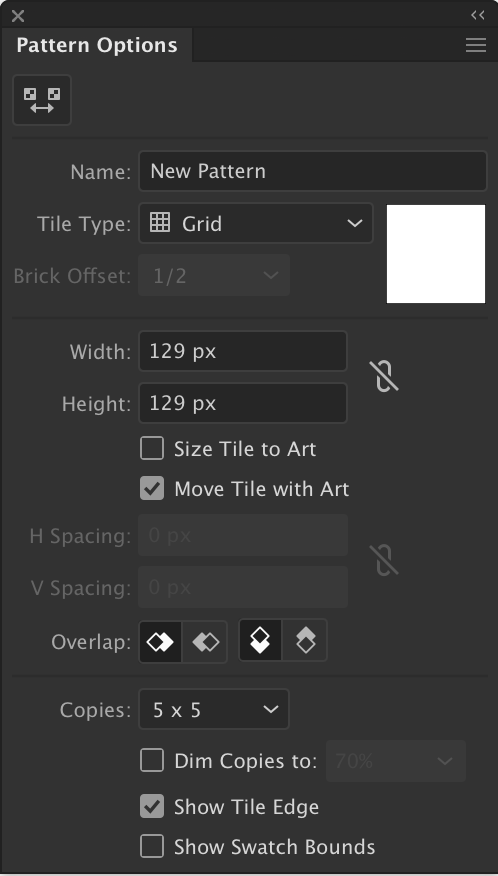
\includegraphics[width=.4\linewidth]{ai-tool}
        \caption{Adobe Illustrator\textsuperscript{\textregistered} \, ``make pattern'' tool.}
        \label{fig:adobe}
    \end{center}
\end{figure}

\section{Practical Applications}

\subsection{Nature}
Like many mathematical subjects, tessellation has manifestations in nature. The most popular natural example is beehive honeycombs in Figure \ref{fig:bee}.

\begin{figure}[H]
    \begin{center}
        \includegraphics[width=.6\linewidth]{honeycomb}
        \caption{Natural honey bee honeycomb, equal to the tessellation of a hexagon.}
        \label{fig:bee}
    \end{center}
\end{figure}

Bees use the hexagonal structure because it offers good structural integrity while also leaving the majority of the surface area of the pattern as empty space, making it perfect for storage and construction. 

\subsection{Art}
Modern art has adopted tessellation as a common element in futuristic and technical looking designs. The most popular tessellations are commonly based on the periodic $\{6,3\}$ hexagonal tessellation. Shown in figure \ref{fig:modern} is an example of a `modern' geometric tessellation. 

\begin{figure}[H]
    \begin{center}
        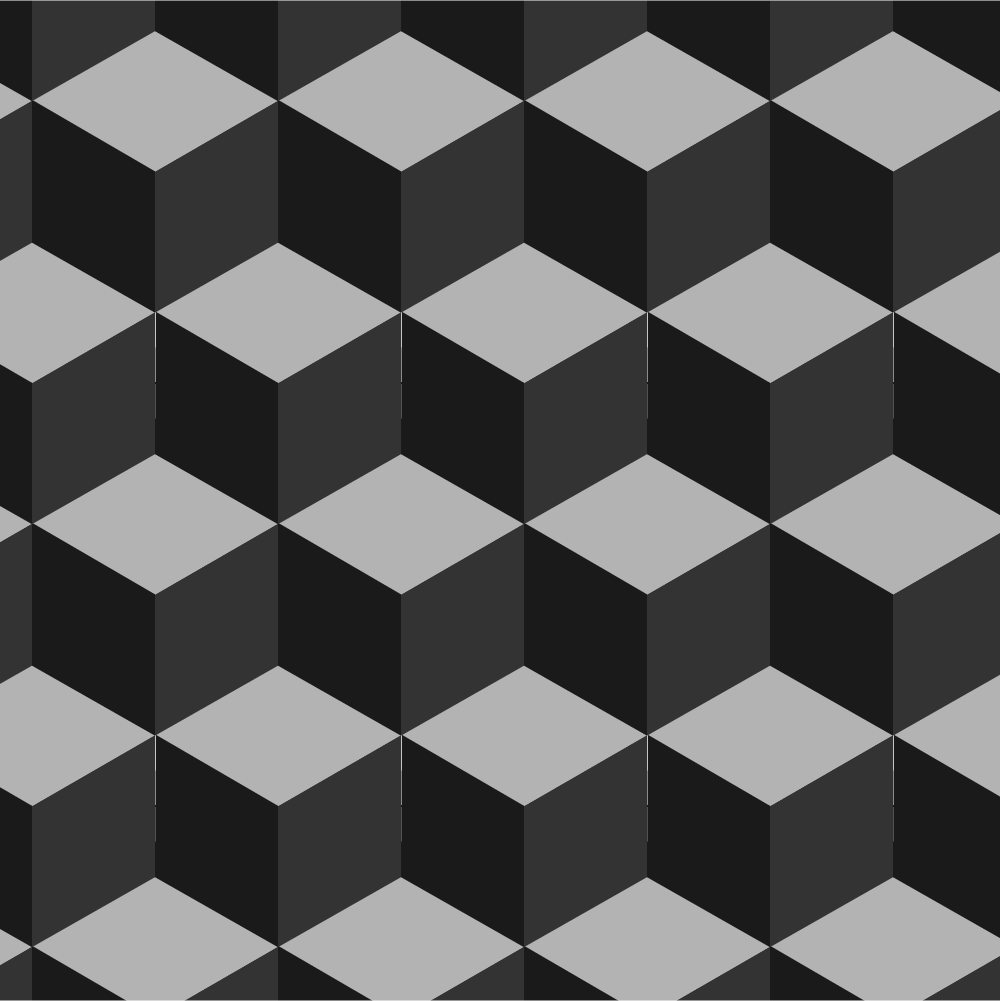
\includegraphics[width=.6\linewidth]{modern-tes}
        \caption{Popular modern $\{6,3\}$ pattern}
        \label{fig:modern}
    \end{center}
\end{figure}

As with the Girih tiles, manipulating the contents of each the base polygon produces different visual styles. The $\{6,3\}$ has been used recently to produce a futuristic or technical aesthetic, and has been adopted by brands associated with technology and engineering such as the Georgia Institute of Technology. 

\subsection{Mechanical Engineering}
As stated before, parts that require few processes to produce and can be used repeatedly instead of multiple configurations are ideal for large scale production and implementation. The tessellation in Figure \ref{fig:square} may have been familiar because it is by far the most common tessellation in the modern world. For most machines, making rectangular objects is the easiest thing to do, next to round objects which cannot be tessellated regularly. 
Tessellation offers a suitable solution for reducing the weight of material without impacting the structural elements of the part. This property of tessellation is why it it frequently used as a hole pattern to make sheet metal parts lighter in the application of robotics. Quadrilateral parallelograms, triangular and hexagonal patterns are the most common in lightening patterns.

\begin{figure}[H]
    \begin{center}
        \caption{Sheet metal plate with a $\{4,4\}$ tessellation pattern}
        \label{fig:belly}
        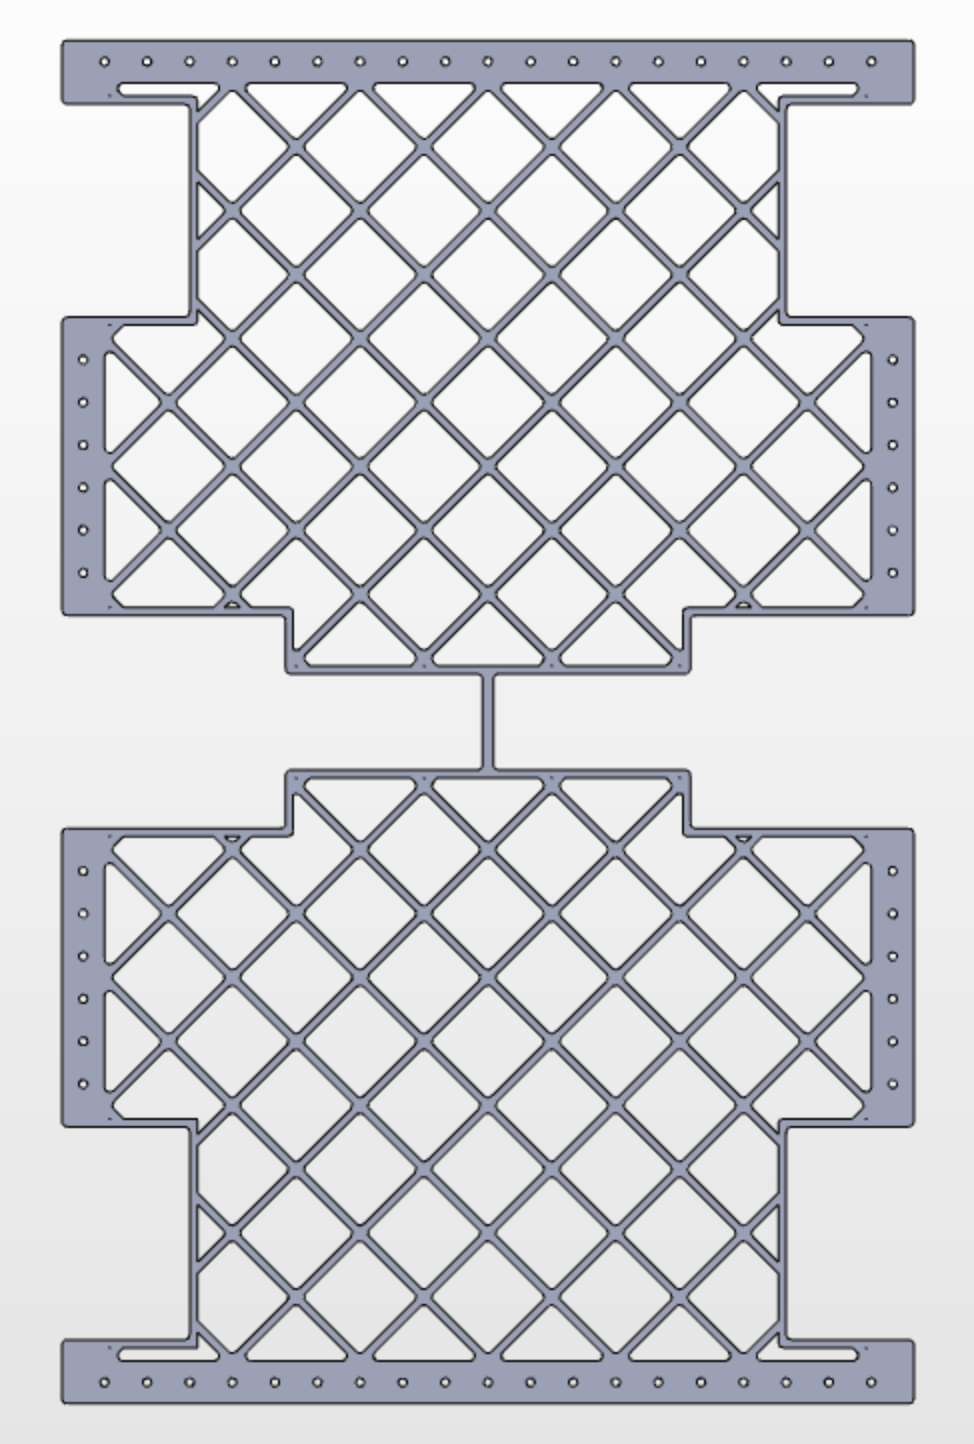
\includegraphics[width=.4\linewidth]{belly}
    \end{center}
\end{figure}

The part shown in Figure \ref{fig:belly} can still distribute compression and tension forces. The application of tessellation patterns in sheet metal part design is one of the main benefits of the material.

Tessellation also benefits manufacturing in the efficient use of materials. Parts can be designed to pack as closely together on a sheet of material and waste as little material as possible, minimizing gaps between shapes. This is exactly what tessellated shapes do. An example of this technique is shown in figure \ref{fig:glasses}.

\begin{figure}[H]
	\begin{center}
		\caption{Cardboard glasses that are designed to minimize wasted material with tessellation.}
		\label{fig:glasses}
		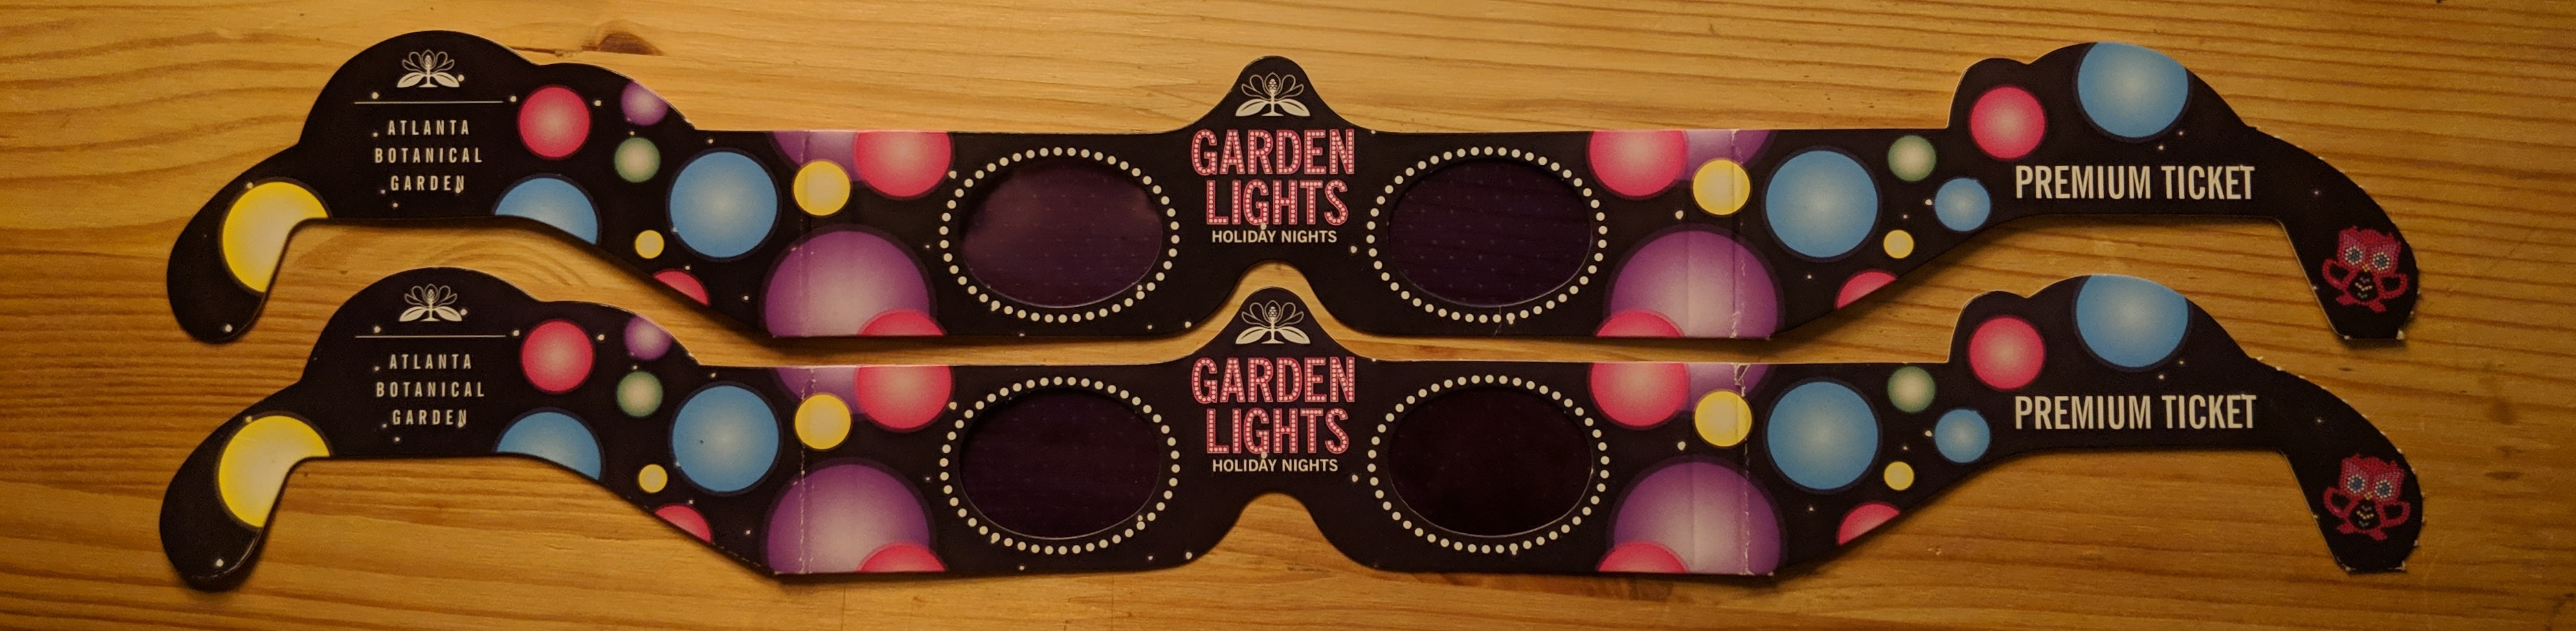
\includegraphics[width=.8\linewidth]{glasses}
	\end{center}
\end{figure}

Notice how the cavity cut out for the nose extends upward from the top of the glasses, which doesn't affect the utility of the glasses, but removes the need to cut away the subtracted material from the nose. Similar material conserving technique is used on the arms of the glasses, but not to the whole extent of removing all waste material. The technically extraneous material on the arms extends into the cavity of the next part in the crevice for the ear. 

\section{Conclusion}

Tessellation offers the best of both worlds in terms of engineering and manufacturing utility as well as aesthetic appeal. It's history in natural structures and decorative applications extends back centuries, and continues to be a prevalent technique in modern graphic design and manufacturing. Tessellated shapes can pack together to minimize or remove waste material entirely. The geometric polygon patterns create a technical visual aesthetic well suited for futuristic graphic design. The mathematics to notate patterns is simple to represent. Most importantly, the patterns are pretty.

\newpage
\bibliography{tynan-math-ia}
\bibliographystyle{apa}

\newpage
\section{Appendix}
\listoffigures

\end{document}